
%%%%%%%%%%%%%%%%%%%%%%%%%%%%%%%%%%%%%%%%%%%%%%%%%%%%%%%%%%%%%%%%%%%%%%%%%%%%%%%%%%%%%%%%
%%
%% DON'T TOUCH ANYTHING !!!
%% edit only files in thesis folder (unless you are upgrading this thesis template)
%%
%%%%%%%%%%%%%%%%%%%%%%%%%%%%%%%%%%%%%%%%%%%%%%%%%%%%%%%%%%%%%%%%%%%%%%%%%%%%%%%%%%%%%%%%

% Language: english, slovak
% Document type: report (master/bachelor thesis)
\documentclass[a4paper,12pt,appendix]{report}

%%
%% Define boolean variables - must be here, don't touch
%%
\usepackage{ifthen}
\usepackage[parfill]{parskip}
\newboolean{english}
\newboolean{bachelor}

%%
%% !!!! edit Author options (thesis style and language)
%%
%%
%% !!!! for MASTER THESIS set to FALSE
%%
\setboolean{bachelor}{false}

%%
%% !!!! for SLOVAK VERSION set to FALSE
%%
\setboolean{english}{false}

%%
%% Formats and Defs
%%

% Packages
\usepackage{epsf}
\usepackage{epsfig}
\usepackage{latexsym}
\usepackage{ucs}
\usepackage{float}
\usepackage[usenames]{color}
\usepackage{newcent}
\usepackage{graphicx}
\usepackage{setspace}
\usepackage{wrapfig}
\onehalfspacing
\usepackage[numbers]{natbib}
%\usepackage{setspace}
\usepackage{url}
\usepackage{eso-pic}

\usepackage{listings}
\usepackage{verbatim}
\usepackage{moreverb}
\usepackage{microtype}
\usepackage[noauto]{chappg}
\usepackage{appendix}
\usepackage{amsmath}

%\usepackage{libertine}

% Language
\ifthenelse {\boolean{english}}
{
	\usepackage[english]{babel}
}
{
	\usepackage{cmap}
	\usepackage[slovak]{babel}
%	\usepackage[IL2]{fontenc}
%	\usepackage[T1]{fontenc}
%	\usepackage{lmodern}
}

%\usepackage{cmap}
%\usepackage[slovak,english]{babel}
\usepackage[T1]{fontenc}
\usepackage[utf8x]{inputenc}
\usepackage{lmodern}

% Section rules
\usepackage{sectsty}
%\usepackage{times}

% Bookmarks

% black references
%\usepackage[pdfborder={0 0 0}]{hyperref} 

% red references
\usepackage[colorlinks=true,linkcolor = blue]{hyperref}

% Colors
\definecolor{light-gray}{gray}{0.95}
\definecolor{gray}{gray}{0.2}
\definecolor{blue}{rgb}{0,0,1}
\definecolor{red}{rgb}{1,0,0}
\definecolor{green}{rgb}{0,0.69,0}
\definecolor{yellow}{rgb}{1,0.35,0}

% Listings settings
\lstdefinelanguage{lua}{
	morekeywords={and,break,do,else,elseif,end,false,for,function,if,in,local,nil,not,or,repeat,return,then,true,until,while},
	morekeywords={[2]arg,assert,collectgarbage,dofile,error,_G,getfenv,getmetatable,ipairs,load,loadfile,loadstring,next,pairs,pcall,print,rawequal,rawget,rawset,select,setfenv,setmetatable,tonumber,tostring,type,unpack,_VERSION,xpcall},
	morekeywords={[2]coroutine.create,coroutine.resume,coroutine.running,coroutine.status,coroutine.wrap,coroutine.yield},
	morekeywords={[2]module,require,package.cpath,package.load,package.loaded,package.loaders,package.loadlib,package.path,package.preload,package.seeall},
	morekeywords={[2]string.byte,string.char,string.dump,string.find,string.format,string.gmatch,string.gsub,string.len,string.lower,string.match,string.rep,string.reverse,string.sub,string.upper},
	morekeywords={[2]table.concat,table.insert,table.maxn,table.remove,	table.sort},
	morekeywords={[2]math.abs,math.acos,math.asin,math.atan,math.atan2,math.ceil,math.cos,math.cosh,math.deg,math.exp,math.floor,math.fmod,math.frexp,math.huge,math.ldexp,math.log,math.log10,math.max,math.min,math.modf,math.pi,math.pow,math.rad,math.random,math.randomseed,math.sin,math.sinh,math.sqrt,math.tan,math.tanh},
	morekeywords={[2]io.close,io.flush,io.input,io.lines,io.open,io.output,io.popen,io.read,io.tmpfile,io.type,io.write,file:close,file:flush,file:lines,file:read,file:seek,file:setvbuf,file:write},
	morekeywords={[2]os.clock,os.date,os.difftime,os.execute,os.exit,os.getenv,os.remove,os.rename,os.setlocale,os.time,os.tmpname},
	keywordstyle=\color{blue}\normalfont,
	ndkeywordstyle=\color{black}\normalfont,
	commentstyle=\color{red}\ttfamily,
	stringstyle=\color{green}\ttfamily,
	identifierstyle=\color{gray},
	sensitive=true,
	morecomment=[l]{--},
	morecomment=[s]{--[[}{]]--},
	morestring=[b]",
	morestring=[d]',
	backgroundcolor=\color{white}, 
	frame=single, 
	frameround=ffff,
	captionpos=b,
	basicstyle=\scriptsize
}

\lstdefinelanguage{nil}{
  identifierstyle=\color{gray},
  sensitive=false,
  columns=flexible,
  backgroundcolor=\color{white}, 
  frame=single, 
  frameround=ffff,
  captionpos=b
}

\lstdefinelanguage{javascript}{
  keywords={typeof, new, true, false, catch, function, return, null, catch, switch, var, if, in, while, do, else, case, break},
  ndkeywords={class, export, boolean, throw, implements, import, this},
  sensitive=false,
  comment=[l]{//},
  morecomment=[s]{/*}{*/},
  morestring=[b]',
  morestring=[b]",
  keywordstyle=\color{blue}\normalfont,
	ndkeywordstyle=\color{black}\normalfont,
	commentstyle=\color{red}\ttfamily,
	stringstyle=\color{green}\ttfamily,
	identifierstyle=\color{gray},
	backgroundcolor=\color{white}, 
	frame=single, 
	frameround=ffff,
	captionpos=b,
	basicstyle=\scriptsize
}

\lstdefinestyle{color}
	{identifierstyle=\color{green}\bfseries, commentstyle=\color{yellow}\bfseries, stringstyle=\color{blue}, keywordstyle=\color{red}\bfseries,morecomment=[l]{\#}}

\lstset{postbreak=\small>>\space, prebreak=\small>>, breakindent=13pt, breaklines=true, inputencoding=utf8x, tabsize=2, showtabs=false, tab=$\to$, style=color, basicstyle=\footnotesize\ttfamily\normalfont, frame=lines, frameround=tttt}

% Figures settings
\usepackage[small,normal,up]{caption2}
\renewcommand{\captionfont}{\small\itshape}
\graphicspath{{figures/}}

%
% this makes list spacing much better.
%
\newenvironment{my_itemize}{
\begin{itemize}
  \setlength{\itemsep}{1pt}
  \setlength{\parskip}{0pt}
  \setlength{\parsep}{0pt}}{
\end{itemize}
}

\newenvironment{my_enumerate}{
\begin{enumerate}
  \setlength{\itemsep}{1pt}
  \setlength{\parskip}{0pt}
  \setlength{\parsep}{0pt}}{
\end{enumerate}
}

\newcommand{\emptyitem}{\item[]}
\newcommand{\myitem}{\item[$-$]}

%Font settings
\makeatletter
\renewcommand{\paragraph}{\@startsection{paragraph}{4}		
{0ex}%
{-3.25ex plus -1ex minus -0.2ex}%
{1.5ex minus 0.2ex}%
 {\normalfont\normalsize\bfseries}}

\makeatother


\stepcounter{secnumdepth}
\stepcounter{tocdepth}

\setcounter{secnumdepth}{3}
\setcounter{tocdepth}{3}

%% Change formating of chapter titles
\usepackage[sf,sl,outermarks]{titlesec}

\ifthenelse {\boolean{bachelor}}
{  
\titleformat{\chapter}
  {\normalfont\Large\bfseries}{\thechapter}{.5em}{\vspace{1ex}}[\titlerule]
\titleformat{\section}
  {\normalfont\large\bfseries}{\thesection}{1em}{}
\titleformat{\subsection}
  {\normalfont\normalsize\bfseries}{\thesubsection}{1em}{}
\titleformat{\subsubsection}
  {\normalfont\normalsize\bfseries}{\thesubsubsection}{1em}{}  
  
\titlespacing*{\chapter}      
	{0pt}{0pt}{15pt}
}
{
\titleformat{\chapter}[display]
  {\normalfont\huge\bfseries}{\chaptertitlename\ \thechapter}{20pt}{\Huge}
\titleformat{\section}
  {\normalfont\Large\bfseries}{\thesection}{1em}{}
\titleformat{\subsection}
  {\normalfont\large\bfseries}{\thesubsection}{1em}{}
\titleformat{\subsubsection}
  {\normalfont\normalsize\bfseries}{\thesubsubsection}{1em}{}
\titleformat{\paragraph}[runin]
  {\normalfont\normalsize\bfseries}{\theparagraph}{1em}{}
\titleformat{\subparagraph}[runin]
  {\normalfont\normalsize\bfseries}{\thesubparagraph}{1em}{}
\titlespacing*{\chapter}      {0pt}{50pt}{40pt}
\titlespacing*{\section}      {0pt}{3.5ex plus 1ex minus .2ex}{2.3ex plus .2ex}
\titlespacing*{\subsection}   {0pt}{3.25ex plus 1ex minus .2ex}{1.5ex plus .2ex}
\titlespacing*{\subsubsection}{0pt}{3.25ex plus 1ex minus .2ex}{1.5ex plus .2ex}
\titlespacing*{\paragraph}    {0pt}{3.25ex plus 1ex minus .2ex}{1em}
\titlespacing*{\subparagraph} {\parindent}{3.25ex plus 1ex minus .2ex}{1em}
}


% What is this ????
\ifthenelse {\boolean{bachelor}}
{
	\sectionfont{\sectionrule{0pt}{0pt}{-2ex}{0.5pt}}
}
{
	\sectionfont{\sectionrule{0pt}{0pt}{-2ex}{0pt}}
}


% Common FIIT stuff
% UAPI
\ifthenelse {\boolean{english}}
	{\newcommand{\UAPI}{Institute of Applied Informatics}}
	{\newcommand{\UAPI}{\'Ustav Aplikovanej Informatiky}}
% UISI
\ifthenelse {\boolean{english}}
	{\newcommand{\UISI}{Institute of Informatics and Software Engineering}}
	{\newcommand{\UISI}{\'Ustav Informatiky a Softvérového Inžinierstva}}
% UPSS
\ifthenelse {\boolean{english}}
	{\newcommand{\UPSS}{Institute of Computer Systems and Networks}}
	{\newcommand{\UPSS}{\'Ustav Počítačových Systémov a Sietí}}

% INFO Bc.
\ifthenelse {\boolean{english}}
	{\newcommand{\INFO}{Informatics}}
	{\newcommand{\INFO}{Informatika}}

\ifthenelse {\boolean{english}}
	{\newcommand{\INFOf}{9.2.1 Informatics}}
	{\newcommand{\INFOf}{9.2.1 Informatika}}

% IS Ing.
\ifthenelse {\boolean{english}}
	{\newcommand{\IS}{Information systems}}
	{\newcommand{\IS}{Informačné systémy}}

\ifthenelse {\boolean{english}}
	{\newcommand{\ISf}{9.2.6 Information systems}}
	{\newcommand{\ISf}{9.2.6 Informačné systémy}}

% SI Ing.
\ifthenelse {\boolean{english}}
	{\newcommand{\SI}{Software Engineering}}
	{\newcommand{\SI}{Softvérové inžinierstvo}}

\ifthenelse {\boolean{english}}
	{\newcommand{\SIf}{9.2.5 Software Engineering}}
	{\newcommand{\SIf}{9.2.5 Softvérové inžinierstvo}}


%%
%% !!!! edit Author details
%%

%%
%% !!!! set your own definitions
%%
\newcommand{\Author}{Michal Fašánek} 
\newcommand{\TitleENG}{Advanced processing of sequential data by artificial neural networks}
\newcommand{\TitleSVK}{Pokročilé spracovanie sekvenčných dát pomocou umelých neurónových sietí}
\newcommand{\Title}{\TitleSVK}
\newcommand{\Supervisor}{Ing. Michal Barla, PhD}
\newcommand{\Year}{2016}
\newcommand{\MonthSVK}{Január}
\newcommand{\MonthENG}{January}
\newcommand{\FIIT}{FIIT-0000-00000}
\newcommand{\Keywords}{Spracovanie dát, neurónové siete}

%%
%% !!!! For UAPI set \UAPI, for other use \UISI, \UPSS
%%
\newcommand{\Place}{\UAPI}

%%
%% !!!! For SI study program set \SI, for other use \IS, \INFO
%% !!!! For SI study field set \SIf, for other use \ISf, \INFOf
%%
\newcommand{\Program}{\IS}
\newcommand{\Field}{\IS}




%%%%%%%%%%%%%%%%%%%%%%%%%%%%%%%%%%%%%%%%%%%%%%%%%%%%%%%%%%%%%%%%%%%%%%%%%%%%%%%%%%%%%%%%

\begin{document}

% Language
\ifthenelse {\boolean{english}}
{
	\renewcommand{\lstlistingname}{Example}
	\renewcommand{\lstlistlistingname}{List of Examples}
	\renewcommand{\bibname}{Bibliography}
	\renewcommand{\appendixname}{Appendix}
	\renewcommand{\appendixtocname}{Appendix}		
}
{
	\renewcommand{\lstlistingname}{Ukážka}
	\renewcommand{\lstlistlistingname}{Zoznam ukážok}	
	\renewcommand{\bibname}{Literatúra}
	\renewcommand{\appendixname}{Príloha}
	\renewcommand{\appendixtocname}{Prílohy}		
}

%%
%% Title Page
%%

%%IMPORTANT
%%%%%%%%%%%%%%%%%%%%%%%%%%%%%%%%%%%%%%%%%%%%%%%%%%%%%%%%%%%%%%%%%%%%%%%%%%%%%%%%%%%%%%%%
%%
%% Front page
%%
%%%%%%%%%%%%%%%%%%%%%%%%%%%%%%%%%%%%%%%%%%%%%%%%%%%%%%%%%%%%%%%%%%%%%%%%%%%%%%%%%%%%%%%%
\begin{center}
\thispagestyle{empty}
\ifthenelse {\boolean{english}}
{
	{\Large Slovak University of Technology in Bratislava}\textbf{}\\
	{\Large Faculty of Informatics and Information Technologies}\textbf{}\\[\baselineskip]
}
{
	{\Large Slovenská technická univerzita v Bratislave}\textbf{}\\
	{\Large Fakulta informatiky a informačných technológií}\textbf{}\\[\baselineskip]
}
{\large \FIIT}\\
\vspace*{4cm}
{\Large \Author}\textbf{}\\[\baselineskip]
{\huge \Title}\textbf{}\\[\baselineskip]
\ifthenelse {\boolean{english}}
{
	\ifthenelse {\boolean{bachelor}}
	{
		{\large Bachelor thesis}\\
	}
	{
		{\large Master thesis}\\
	}
}
{
	\ifthenelse {\boolean{bachelor}}
	{
		{\large Bakalárska práca}\\
	}
	{
		{\large Diplomová práca}\\
	}
}

\end{center}
\vspace{\stretch{1}}
\ifthenelse {\boolean{english}}
{
	Supervisor: \Supervisor \\\\
	\Year,\ \MonthENG 
}
{
	Vedúci práce: \Supervisor \\\\
    \MonthSVK,\ \Year
}

%%%%%%%%%%%%%%%%%%%%%%%%%%%%%%%%%%%%%%%%%%%%%%%%%%%%%%%%%%%%%%%%%%%%%%%%%%%%%%%%%%%%%%%%
%%
%% Title page
%%
%%%%%%%%%%%%%%%%%%%%%%%%%%%%%%%%%%%%%%%%%%%%%%%%%%%%%%%%%%%%%%%%%%%%%%%%%%%%%%%%%%%%%%%%
\newpage
\begin{center}
\thispagestyle{empty}
\ifthenelse {\boolean{english}}
{
	{\Large Slovak University of Technology in Bratislava}\textbf{}\\
	{\Large Faculty of Informatics and Information Technologies}\textbf{}\\[\baselineskip]
}
{
	{\Large Slovenská technická univerzita v Bratislave}\textbf{}\\
	{\Large Fakulta informatiky a informačných technológií}\textbf{}\\[\baselineskip]
}
{\large \FIIT}\\
\vspace*{4cm}
{\Large \Author}\textbf{}\\[\baselineskip]
{\huge \Title}\textbf{}\\[\baselineskip]
\ifthenelse {\boolean{english}}
{
	\ifthenelse {\boolean{bachelor}}
	{
		{\large Bachelor thesis}\\
	}
	{
		{\large Master thesis}\\
	}
}
{
	\ifthenelse {\boolean{bachelor}}
	{
		{\large Bakalárska práca}\\
	}
	{
		{\large Diplomová práca}\\
	}
}
\end{center}
\vspace{\stretch{1}}
\ifthenelse {\boolean{english}}
{
	\textrm{
	    \begin{normalsize}
	    \begin{flushleft}
	    \begin{tabular}{ll}
			Study program: & \Program\\ 
			Field of study: & \Field\\
			Place: & \Place\\
			Supervisor: & \Supervisor \\
			\Year,\ \MonthENG
	    \end{tabular}
	    \end{flushleft}
	  \end{normalsize}
	}		
}
{
	\textrm{
	    \begin{normalsize}
	    \begin{flushleft}
	    \begin{tabular}{ll}
			Študijný program: & \Program\\ 
			Študijný odbor: & \Field\\
			Miesto vypracovania: & \Place\\
			Vedúci práce: & \Supervisor \\
		    \MonthSVK,\ \Year
	    \end{tabular}
	    \end{flushleft}
	  \end{normalsize}
	}	
}



%%
%% Empty page for assigment
%%
%\newpage
\thispagestyle{empty}
\vspace*{9cm}
\begin{center}
{\color{red}\LARGE{$>>>>$ ASSIGNMENT $<<<<$\\$>>>>$ ZADANIE $<<<<$}}
\end{center}

%%
%% Anotation
%%
\pagenumbering{roman}
\setcounter{page}{2}

%%%%%%%%%%%%%%%%%%%%%%%%%%%%%%%%%%%%%%%%%%%%%%%%%%%%%%%%%%%%%%%%%%%%%%%%%%%%%%%%%%%%%%%%
%%
%% Slovak annotation
%%
%%%%%%%%%%%%%%%%%%%%%%%%%%%%%%%%%%%%%%%%%%%%%%%%%%%%%%%%%%%%%%%%%%%%%%%%%%%%%%%%%%%%%%%%
\newpage
\thispagestyle{plain}
\begin{center}
\begin{Large}
\textbf{Anotácia} \\
\end{Large}
\end{center}
Slovenská technická univerzita v Bratislave \\
FAKULTA INFORMATIKY A INFORMAČNÝCH TECHNOLÓGIÍ 
\noindent
	\textrm{
	    \begin{normalsize}
	    \begin{flushleft}
	    \begin{tabular}{@{}lp{0.7\textwidth}@{}}
			Študijný program: & \Program\\ 
			\ifthenelse {\boolean{bachelor}}{{Bakalárska práca: }}{{Diplomová práca: }} & \TitleSVK \\
			Autor: & \Author \\
			Vedúci práce: & \Supervisor \\
			\MonthSVK,\ \Year
	    \end{tabular}
	    \end{flushleft}
	  \end{normalsize}
	}
\noindent
\\
%%%%%%%%%%%%%%%%%%%%%%%%%%%%%%%%%%%%%%%%%%%%%%%%%%%%%%%%%%%%%%%%%%%%%%%%%%%%%%%%%%%%%%%%
%%
%% Slovak annotation
%%
%%%%%%%%%%%%%%%%%%%%%%%%%%%%%%%%%%%%%%%%%%%%%%%%%%%%%%%%%%%%%%%%%%%%%%%%%%%%%%%%%%%%%%%%
Analýza dát z používateľského správania k zdrojom na webe je v súčasnosti populárna téma, vzhľadom na svoj potenciál zlepšovať služby poskytované návštevníkom webu. Najnovšie prístupy skúmajú aj možnosti aplikácie metód strojového učenia. 
V tejto práci sa zameriavam na možnosti využitia rekurentných neurónových sietí s dlhou krátkodobou pamäťou(LSTM) pri analýze dát z platobných brán pre používanie online spravodajských portálov. Takáto analýza poskytuje náhľad do používateľského správania a z toho vyplývajúce možnosti spätnej väzby voči návštevníkom online spravodajských portálov. Manažment biznisu orientovaného na služby si čoraz viac uvedomuje cenu verného zákazníka na trhu. Je preto nutné odhaliť zákazníka uvažujúceho o prechode ku konkurencii pomocou jeho správania  a pozitívne motivovať jeho vernosť.




%%%%%%%%%%%%%%%%%%%%%%%%%%%%%%%%%%%%%%%%%%%%%%%%%%%%%%%%%%%%%%%%%%%%%%%%%%%%%%%%%%%%%%%%
%%
%% English annotation
%%
%%%%%%%%%%%%%%%%%%%%%%%%%%%%%%%%%%%%%%%%%%%%%%%%%%%%%%%%%%%%%%%%%%%%%%%%%%%%%%%%%%%%%%%%
\newpage
\thispagestyle{plain}
\begin{center}
\begin{Large}
\textbf{Annotation} \\
\end{Large}
\end{center}
Slovak University of Technology Bratislava \\
FACULTY OF INFORMATICS AND INFORMATION TECHNOLOGIES 
\noindent
	\textrm{
	    \begin{normalsize}
	    \begin{flushleft}
	    \begin{tabular}{@{}lp{0.7\textwidth}@{}}
			Study program: & \Program\\ 
			\ifthenelse {\boolean{bachelor}}{{Bachelor thesis: }}{{Master thesis: }} & \TitleENG \\
			Author: & \Author \\
			Supervisor: & \Supervisor \\
			\Year,\ \MonthENG
	    \end{tabular}
	    \end{flushleft}
	  \end{normalsize}
	}
\noindent
\\
%%%%%%%%%%%%%%%%%%%%%%%%%%%%%%%%%%%%%%%%%%%%%%%%%%%%%%%%%%%%%%%%%%%%%%%%%%%%%%%%%%%%%%%%
%%
%% English annotation
%%
%%%%%%%%%%%%%%%%%%%%%%%%%%%%%%%%%%%%%%%%%%%%%%%%%%%%%%%%%%%%%%%%%%%%%%%%%%%%%%%%%%%%%%%%
Recommender systems are used to generate additional value from data that is constantly created by user access to the online services and products. Such recommendations can improve online business and customer experience from accessing system. new methods research possibilities of applying machine learning to improve these recommendations.
In this paper I focus on using recurrent neural networks with long short-term memory(LSTM) in data analysis from electronic portals providing online products and services. Such analysis lets us peer into the behavior of users and the possibility of feedback it creates. Management of customer-oriented business is realizing value of loyal customer more than ever before on this competitive market. It is therefore necessary to generate only relevant recommendations that do not annoy or spam customers, which might decrease their willingness for return.



%%
%% Declaration
%%
%%%%%%%%%%%%%%%%%%%%%%%%%%%%%%%%%%%%%%%%%%%%%%%%%%%%%%%%%%%%%%%%%%%%%%%%%%%%%%%%%%%%%%%%%
%%
%% DECLARATION
%%
%%%%%%%%%%%%%%%%%%%%%%%%%%%%%%%%%%%%%%%%%%%%%%%%%%%%%%%%%%%%%%%%%%%%%%%%%%%%%%%%%%%%%%%%
Lorem ipsum dolor sit amet, consectetur adipisicing elit, sed do eiusmod tempor incididunt ut labore et dolore magna aliqua....\\


%%
%% Contents
%%
%\pagestyle{empty}
\newpage
\tableofcontents{}

%%
%% Lists
%%
% \newpage
% List of Figures
 %\listoffigures  
 %\newpage
% List of Tables
 %\listoftables
 %\newpage
% List of Listings
% \lstlistoflistings


%%
%% Clear Page And Set New Page Counter
%%
\clearpage
\pagenumbering{arabic}
\setcounter{page}{1}

%%
%% Thesis 
%%

%%%%%%%%%%%%%%%%%%%%%%%%%%%%%%%%%%%%%%%%%%%%%%%%%%%%%%%%%%%%%%%%%%%%%%%%%%%%%%%%%%%%%%%%
%%
%% This is a recomended minimal thesis structure, add aditional chapters in the following files
%%
%%%%%%%%%%%%%%%%%%%%%%%%%%%%%%%%%%%%%%%%%%%%%%%%%%%%%%%%%%%%%%%%%%%%%%%%%%%%%%%%%%%%%%%%

%%
%% Introduction
%%
\newpage
\chapter{Úvod}

Lorem ipsum dolor sit amet, consectetuer adipiscing elit, sed diam nonummy nibh euismod tincidunt ut laoreet dolore magna aliquam erat volutpat. Ut wisi enim ad minim veniam, quis nostrud exerci tation ullamcorper suscipit lobortis nisl ut aliquip ex ea commodo consequat.

Duis autem vel eum iriure dolor in hendrerit in vulputate velit esse molestie consequat, vel illum dolore eu feugiat nulla facilisis at vero eros et accumsan et iusto odio dignissim qui blandit praesent luptatum zzril delenit augue duis dolore te feugait nulla facilisi. Nam liber tempor cum soluta nobis eleifend option congue nihil imperdiet doming id quod mazim placerat facer possim assum. Typi non habent claritatem insitam; est usus legentis in iis qui facit eorum claritatem. Investigationes demonstraverunt lectores legere me lius quod ii legunt saepius. 

Claritas est etiam processus dynamicus, qui sequitur mutationem consuetudium lectorum. Mirum est notare quam littera gothica, quam nunc putamus parum claram, anteposuerit litterarum formas humanitatis per seacula quarta decima et quinta decima. Eodem modo typi, qui nunc nobis videntur parum clari, fiant sollemnes in futurum.

%%
%% Analysis
%%
\newpage
\chapter{Analýza}
\label{ch:Analýza}
V tejto časti sa venujeme dôkladnej analýze podkladov. Jednotlivé časti sú popísané v rozsahu relevantnom pre túto prácu. Analýza je štrukturovaná na nasledovné časti:

\begin{my_itemize}
	\item {Problémová oblasť}
	\item {Dáta sprístupnené pre prácu}
	\item {Neurónové siete}
	\item {Výskum v danej oblasti}
\end{my_itemize}

\section{Problémová oblasť}
\label{analyza_problemova_oblast}

V tejto práci sa zameriavame na predikciu úbytku zákazníkov(churn rate) pri predplatiteľských službách. V súčasnej dobe sa do popredia biznis prístupov stále viac dostávajú prístupy riadenia vzťahov zo zákazníkmi(customer relationship management). Ukazuje sa totiž, že na trhu s dostatočným pokrytím poskytovateľov cieľovej služby je niekoľkonásobne drahšie získať nového ako udržať si existujúceho zákazníka. Tento prístup však vyžaduje rozsiahlu znalosť dostupnej zákazníckej základne, ktorou poskytovateľ disponuje. \newline

\subsection{Predikcia úbytku zákazníkov}
\label{analyza_ubytok_zakaznikov}

Predikcia úbytku zákazníkov sa venuje spracovaniu dostupných dát o zákazníckej aktivite, službách ktoré využívajú a vývoja ich správania v čase. Takéto dáta  Výsledkom analýzy je štatistika poskytujúca informácie o jednotlivých zákazníkoch a ich šanci na presun k inému poskytovateľovi. Z týchto dát je následne odvoditeľné, aké percento zákazníkov odíde ku konkurencii a aký to bude mať dopad na finančné príjmy od ktorých je poskytovateľ závislý. 

\subsection{Moderovanie úbytku zákazníkov}
\label{analyza_moderovanie_ubytku}

Vo vzťahu k úbytku zákazníkov definuje CRM dva základné prístupy, ktorými je možné moderovať úbytok. 

\subsubsection{Reaktívny prístup}
\label{analyza_reaktivny_pristup}

Motivácia zákazníka pre zotrvanie s pôvodným poskytovateľom služby nastáva, až keď sa zákazník explicitne rozhodne pre prechod ku konkurenčnému poskytovateľovi. V tomto okamihu začína poskytovateľ na svojho zákazníka apelovať výhodnými ponukami, zľavami alebo inými spôsobmi motivácie pre zotrvanie u poskytovateľa. Takýto prístup sa ukazuje ako ľahko zneužiteľný ostatnými zákazníkmi, ktorí by inak nemali motiváciu pre prechod ku konkurencii. Predikcia úbytku zákazníkov v tomto prístupe nemá nijakú významnú úlohu.

\subsubsection{Proaktívny prístup}
\label{analyza_proaktivny_pristup}

Pri úspešnej predikcii záujmu zákazníka o prechod ku konkurenčnému poskytovateľovi je možné efektívne jeho zámer smerovať pozitívnou motiváciou. Tento prístup však predpokladá vysokú úspešnosť predikčných metód. Pri nesprávnej identifikácii zákazníckeho správania je totiž možné nielen nezabrániť zákazníkom v presune ku konkurenčnému modelu, ale aj investícii finančných prostriedkov do skupiny zákazníkov, ktorá by naďalej generovala zisk aj bez významnejšej motivácie, resp. nevrátila by rozdielom v úbytku motivačné náklady, ktoré na ňu daný poskytovateľ vynaložil.

\section{Dáta sprístupnené pre prácu}
\label{analyza_data}

Pre túto prácu boli sprístupnené dáta z platobnej brány portálu pre online spravodajské denníky. Platobný portál poskytuje platformu pre periodiká, ktoré majú záujem o online funkcionalitu ale nemajú záujem implementovať vlastný platobný systém. Zákazníci tohto portálu tak získavajú rýchle riešenie pre možnosť vyhradenia exkluzívneho obsahu zo svojich online materiálov.

\subsection{Exkluzívny obsah}
\label{analyza_exkluzivny_obsah}

Exkluzívny obsah je nástroj, ktorý množstvo poskytovateľov služieb využíva pri prechode na web. Umožňuje prístup k väčšiemu počtu potenciálnych zákazníkov, pričom poskytovateľovi ostáva možnosť oddeliť, čo bude prístupné každému od exkluzívneho obsahu určeného pre predplatiteľov. \newline
Realizáciu exkluzívneho obsahu pomocou platobnej brány tretej strany umožňuje špecifikácia VAW(value added web). VAW aplikuje TINA(Telecommunications Information Networking Architecture) biznis model do klasického WWW(world wide web) prostredia.  Určuje tak vzťahy medzi jednotlivými právnymi subjektami podľa obr.~\ref{fig:vaw}. Poskytovateľ služieb(spravodajské periodikum) tak môže poskytovať nielen klasický ale aj exkluzívny obsah bez toho, aby sa vo väčšej miere muselo zaoberať správou poskytovaných služieb a finančnou administratívou. Za tú zodpovedá sprostredkovateľ(platobný portál), ktorého úloha spočíva v správe exkluzívneho obsahu vo vzťahu ku koncovému používateľovi.

\begin{figure}[H]
\begin{center}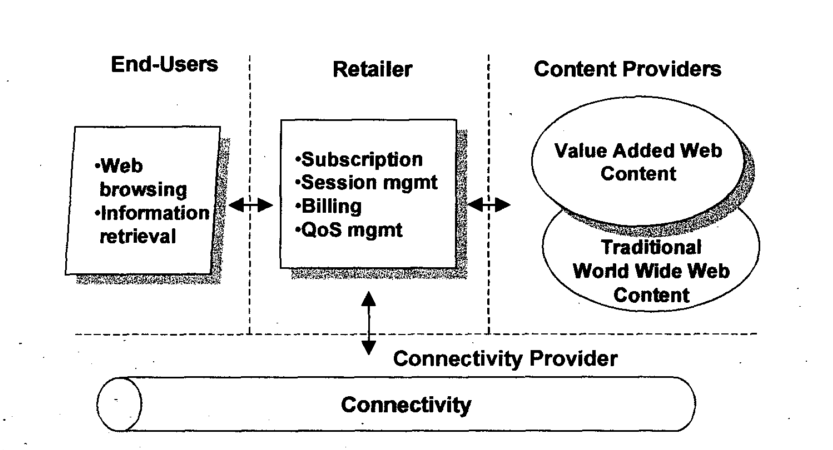
\includegraphics[scale=0.48]{vaw}\end{center}
\caption[vaw]{Základná schéma VAW}\label{fig:vaw}
\end{figure}

\subsection{Získavanie dát}
\label{analyza_ziskavanie_dat}

Pri pokuse o prístup k exkluzívnemu obsahu stojí medzi používateľom a obsahom platobná brána portálu. Používateľovi bez predplatenej služby je zobrazená ponuka na platený prístup. Predplatitel prechádza cez bránu a je mu sprístupnený exkluzívny obsah. Pri všetkých aktivitách na portáli sú zaznamenávané používateľské údaje. Dostupné údaje sú vo forme záznamov - textových súborov priebežne generovaných používateľskou činnosťou. 
Bežná činnosť pri analýze záznamov z činnosti a práci s velkými dátami všeobecne je predspracovanie dát. Pri sledovaní činnosti používateľov sa generujú súbory so stovkami miliónov až miliardami záznamov. V súčasnosti nie je možné klasickými prístupmi spracovať takéto objemy dát bez predspracovania - filtrovania, segmentácie a čistenia dát. Spôsob predspracovania dát je z podstatnej časti ovplyvnený metódami, ktorými chceme dáta spracovať. Pri práci so záznamami je bežné deliť dáta na tzv. používateľské prístupy (user sessions). Používateľský prístup modeluje aktivitu - jeden prístup jedného používateľa. Všeobecne platí, že ak používateľ dosiahne v činnosti pauzu 30 a viac minút, jedná sa o samostatný nový prístup. Takto rozdelené záznamy poskytujú elasticitu pri spracovaní podľa špecifického času alebo podľa používatelov. 

Medzi najdôležitejšie dostupné údaje z platobného portálu patria:

\begin{my_itemize}
	\item {IP adresa}
	\item {Používateľský účet}
	\item {Časový rozsah prístupu}
	\item {Prehliadaný obsah}
	\item {Aktivácia/prerušenie predplatného}
\end{my_itemize}

\section{Neurónové siete}
\label{analyza_neuronove_siete}
%citovat deeplearning.org

Koncept neurónových sietí vznikol v 40. rokoch minulého storočia inšpiráciou biologickými neurónovými sieťami v mozgu. Cieľom bolo prekonať bariéru medzi tým, čo je pre ľudský mozog ľahko riešitelné ale ťažko formálne definovatelné matematickými pravidlami. Tieto problémy, ktoré riešime intuitívne, pri pokuse o formálnu špecifikáciu ukazujú, aké množstvo znalostí používame v každodennom živote. Ako vhodný príklad slúži vizuálne rozoznávanie objektov, ktoré je pre osobu samozrejmé, no až v posledných rokoch zaznamenávame prvé úspechy v tejto problematike.  

\subsection{Štruktúra}
\label{analyza_struktura_nn}

Podobne ako v mozgu, základ neurónovej siete tvoria neuróny a prepojenia medzi nimi. Neuróny sú organizované vo vrstvách, ktoré sa delia na 3 základné typy. 
%\newline
\noindent

\textbf{Vstupná vrstva} - reprezentuje dáta, ktoré podsúvame sieti pre interpretáciu. Dáta musia byť pred posunutím vstupnej vrstve často predspracované, aby bola sieť schopná interpretovať ich. Počet neurónov na vstupnej vrstve je ovplyvnený množstvom dát, ktoré máme na vstupe. V sieti existuje iba jediná vstupná vrstva.
%\newline
\noindent

\textbf{Výstupná vrstva} - interpretácia dát neurónovou sieťou. Výstupnú vrstvu je možné nazvať ,,výsledok"  siete. Jedná sa o jedinú vrstvu s obvykle jediným neurónom.  
%\newline
\noindent

\textbf{Skrytá vrstva} - nachádzajú sa medzi vstupnou a výstupnou vrstvou. Ich počet určuje dĺžku modelu. Sieť nemusí mať ani jednu skrytú vrstvu, no takáto sieť dokáže modelovať iba lineárnu závislosť. Všeobecne platí, že čím viac skrytých vrstiev má sieť, tým zložitejšie vzťahy dokáže simulovať. Zvyšujú sa však aj nároky na učenie a výpočtové nároky. Jediná skrytá vrstva vytvára pozoruhodný rozdiel v aplikovatelnosti modelu, keďže prekonáva hranicu lineárnej závislosti funkcie, ktorú model pokrýva. Pri vysokej zložitosti modelu je možné naraziť na problém preučenia, ktorý bráni sieti korektne generalizovať. Neexistuje nijaký spoľahlivá metóda pre správny počet alebo veľkosť skrytých vrstiev. Empiricky sa vyvinulo niekoľko odhadov, ale v praxi je nutné overovať správnosť modelu praktickou evaluáciou. Odhadové pravidlá najčastejšie padajú na neschopnosti integrovať vo svojom rozhodnutí komplexitu úlohy a redundanciu v tréningových dátach.
%\newline
\noindent

\textbf{Prepojenia} - Váhované prepojenia medzi neurónmi fungujú ako pamäť neurónovej siete. V jednoduchom modeli neurónovej siete sú prepojenia iba medzi neurónmi navzájom susediacich vrstiev. Prepojenie existuje medzi každým neurónom \textit{n}-tej do \textit{n+1} vrstvy. Neuróny jednej vrstvy pritom medzi sebou nie sú prepojené. Signál sa šíri týmito prepojeniami od vstupnej vrstvy smerom k výstupnej vrstve v jednom smere, ako je to ilustrované na obr.~\ref{fig:fnn}. Takéto siete sa volajú \textit{dopredné}. Hlavný účel prepojenia je niesť váhu. Váha prepojenia určuje, aký významný je vzťah medzi dvomi danými neurónmi, ktoré spája. Korektná váha daného prepojenia je na začiatku neznáma, jej korektné nastavenie je výsledkom procesu učenia.
%\newline
\noindent

\textbf{Neurón} - predstavuje základnú stavebnú jednotku neurónovej siete. Skladá sa z \textit{aktivačnej funkcie} a \textit{prahovej hodnoty}. Prahová hodnota neurónu je pripočítaná k sume vstupných váhovaných hodnôt. Na výsledok sa následne aplikuje aktivačná funkcia. Takýto výstup je následne prepojeniami posielaný do ďaľších neurónov. Špeciálny prípad je neurón vstupnej a výstupnej vrstvy. Na vstupe totiž neurón hodnotu iba posiela ďalej a na výstupe po spracovaní nie je zasielaná nikam - predstavuje výsledok siete.
%\newline
\noindent


%citovat a tutorial on training reccurent NN z mendeleya
\begin{figure}[H]
\begin{center}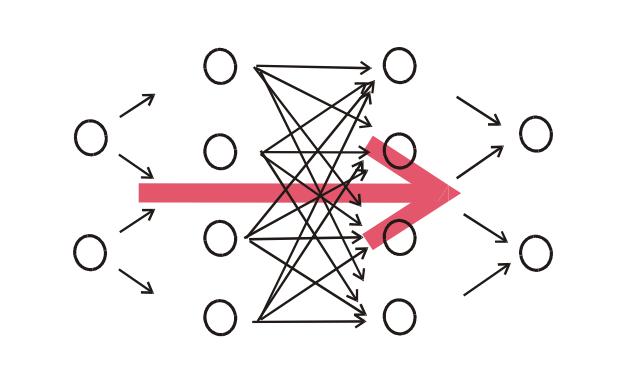
\includegraphics[scale=0.64]{fnn}\end{center}
\caption[fnn]{Štruktúra doprednej neurónovej siete}\label{fig:fnn}
\end{figure}

\subsection{Učenie neurónovej siete}
\label{analyza_ucenie_nn}

Učenie predstavuje kľúčovú aktivitou pre schopnosť siete produkovať požadované výsledky. Spočíva vo vystavovaní neurónovej siete tréningovým dátam, ktoré sa sieť snaží interpretovať.

 %semi-supervidsed learning, active learning, reinforced learning
\textbf{Učenie s učiteľom} je metóda, pri ktorej je dostupná sada tréningových dát ,,označená". Pri interpretovaní výsledku je možné okamžite určiť, aká chyba nastala a následne ju propagovať do siete. Na toto sa využíva tzv. \textit{spätná propagácia}, ktorá upravuje váhy siete v rozsahu chyby, ktorá nastala - rozdiel medzi správnym výsledkom pre daný vstup a samotným výsledkom siete.
\noindent

\textbf{Učenie bez učiteľa} predstavuje alternatívnu metódu, pri ktorej tréningové dáta nemajú dostupné výsledky. Neurónová sieť sa sama učí rozhodnúť, čo je pre ňu relevantné. Učenie bez učiteľa predstavuje možnosť ako získať takmer neobmedzené množstvá tréningových dát tam, kde učenie s učiteľom vyžaduje manuálne a kvôli časovej náročnosti nedostupné označovanie.
\noindent

%deeplearning.org
\subsection{Hyperparametre}
\label{analyza_hyperparametre}

Nastavenia, pomocou ktorých kontrolujeme správanie neurónových sietí sa nazývajú \textit{hyperparametre}. Tieto hodnoty nie sú získané učením siete pokiaľ nemodelujeme vnorený systém za týmto účelom. Príkladom hyperparametra je počet skrytých vrstiev neurónovej siete. Pri nízkom počte nebude model schopný naučiť sa funkciu definovanú problémom. Pri vysokom počte je možné, že sieť v sebe uloží menší tréningový dataset, nazývané tiež ako problém \textit{preučenia}. Pri preučení sieť nezíska schopnosť generalizácie problému kvôli sledovaniu tréningového datasetu. Je zjavné, že zvolenie správnych hyperparametrov má pre výsledky metódy kľúčovú úlohu. Medzi ďaľšie významné hyperparametre patria:
\begin{my_itemize}
	\item {Šírka jednotlivých vrstiev}
	\item {Rýchlosť učenia}
	\item {Momentum}
	\item {Aktivačné funkcie neurónov}
\end{my_itemize}


%citovat a tutorial on training reccurent NN z mendeleya a deeplearning org
\subsection{Rekurentné neurónové siete}
\label{analyza_pokrocile_modely_nn}

Do popredia výskumu sa v súčasnosti dostávajú pokročilé modely, ktoré už nie sú obmedzené na jednoduchý dopredný prístup. Vďaka rapídnemu zvyšovaniu výkonu grafických kariet sa čoraz častejšie aplikujú rekurentné modely neurónových sietí. Špecializáciou rekurentných sietí je práca so sekvenčnými dátami. Tieto siete predstavujú generalizáciu dopredných modelov ich rozšírením o cyklické prepojenia. Takýmto spôsobom je možné využiť súčasnú hodnotu premennej na ovplyvnenie vlastnej hodnoty v budúcnosti. Cyklický charakter rekurentného modelu je zobrazený na obr.~\ref{fig:rnn}.

%citovat a tutorial on training reccurent NN z mendeleya
\begin{figure}[H]
\begin{center}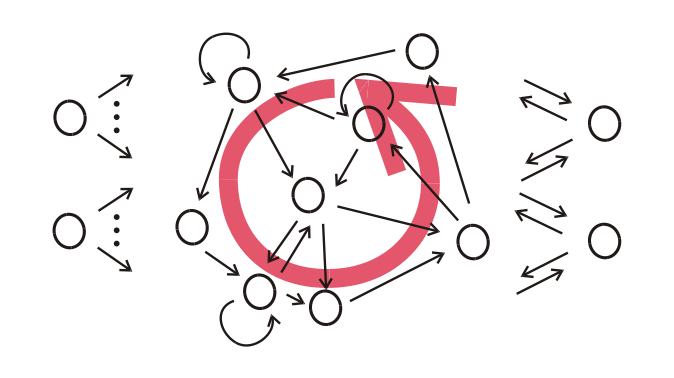
\includegraphics[scale=0.64]{rnn}\end{center}
\caption[rnn]{Štruktúra rekurentnej neurónovej siete}\label{fig:rnn}
\end{figure}

\subsection{Siete s dlhou krátkodobou pamäťou - LSTM}

%perfektne zdroje k LSTM aj odkazy v deeplearning.org pdf
LSTM predstavuje vylepšený model klasickej RNN. Vnútorná štruktúra ako doplnok ku externej rekurencii medzi jednotlivými neurónmi obsahuje aj \textit{internú rekurenciu}, zobrazenú v štruktúre LSTM neurónu na obr.~\ref{fig:lstm}. Medzi najdôležitejšie súčasti tohto modelu patria sigmoidné brány, ktoré rozhodujú o tom, ako sa signál bude širiť.
\newline
\textbf{Brána zabudnutia} ovplyvňuje, či nastáva vnútorná rekurencia neurónu. Stav tak môže ale nemusí byť faktorom ovplyvňujúcim nasledujúcu iteráciu výpočtu v sieti. Významné zlepšenie v LSTM sieťach prišlo s myšlienkou \textit{kontextom podmieneného zabúdania}. Takýto model sa ukazuje extrémne výhodným pri riešení problémov zahŕňajúcich \textit{časové pauzy(lags)}.
%citovat "Learning precise timing with LSTM"
 Dôležitý prvok  na obr.~\ref{fig:lstm} predstavuje čierna kocka. Označuje pauzu o veľkosti jednej iterácie. Hodnota signálu tak ovplyvňuje nasledujúcu iteráciu, tj. vplýva na neskoršie udalosti.
\newline
\noindent

LSTM siete v praxi dokázali svoje schopnosti pri aplikácií na rôzne netriviálne dátové problémy. Pozornosť je kladená na frekventovanú časovú závislosť v dátach:
%deeplearning LSTM ma odkazy na konkretne projekty
\begin{my_itemize}
	\item{Rozoznávanie rukopisu}
	\item{Generovanie rukopisu}
	\item{Rozoznávanie reči}
	\item{Označovanie obrázkov}
\end{my_itemize}

%deeplearning org
\begin{figure}[H]
\begin{center}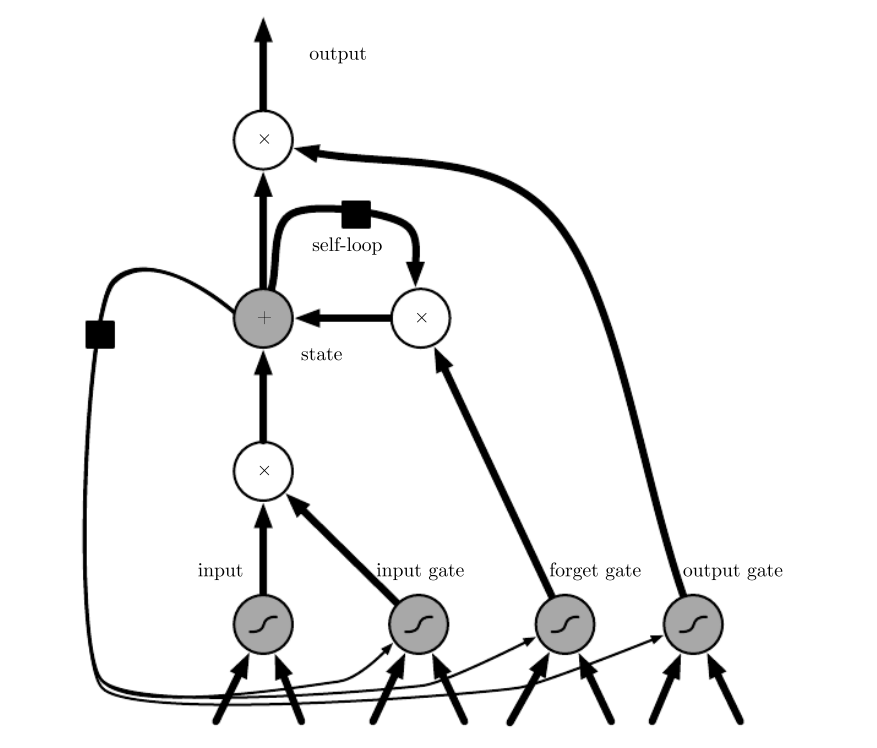
\includegraphics[scale=0.64]{lstm}\end{center}
\caption[lstm]{Štruktúra LSTM bunky}\label{fig:lstm}
\end{figure}

\section{Výskum v danej oblasti}
\label{analyza_vyskum_danej_oblasti}

\begin{comment}
\section{Časť}
\label{sec:Časť}
V tejto časti sa venujeme 
\begin{figure}[H]
\begin{center}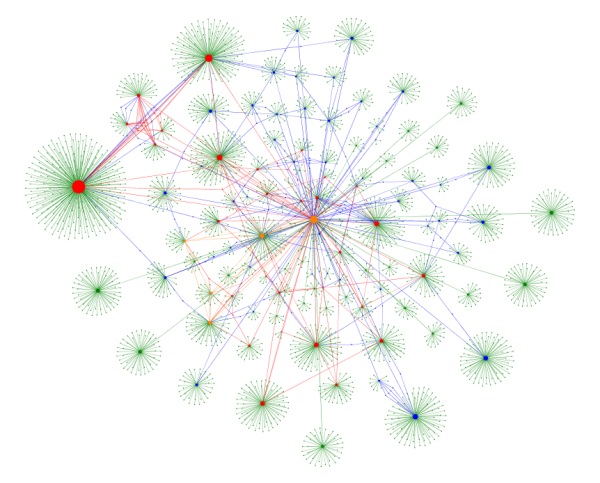
\includegraphics[scale=0.48]{figure}\end{center}
\caption[Name figure]{Name figure}\label{fig:figure}
\end{figure}

%\subsection{Enumeration}
\subsection{Číslovaný zoznam}
\begin{my_enumerate}
	\item {cieľ 1}
	\begin{my_enumerate}
		\item {cieľ 1.a}
		\item {cieľ 1.b}
	\end{my_enumerate}
	\item {cieľ 2}
	\item {cieľ 3}
\end{my_enumerate}

%\subsection{Citation}
\subsection{Citácia}
Lorem ipsum dolor sit amet, consectetuer adipiscing elit, sed diam nonummy nibh euismod tincidunt ut laoreet dolore magna aliquam erat volutpat~\cite{1}.

%\subsection{Labels \& References}
\subsection{Návestia \& Referencie}
Viď. sekcia~\ref{sec:Príklady}.\\
Viď. ukážka~\ref{fig:ukážka}.\\
Viď. číslovanie~\ref{lst:metrics_LOC}.\\
Viď. tabuľka~\ref{tab:tabuľka1}.

%\subsection{Examples}
\subsection{Príklady}
\label{sec:Príklady}

\begin{lstlisting}[ language=html, caption={Príklad 1}, label={lst:metrics_LOC},
	keywordstyle=\color{blue}\bfseries,
	ndkeywordstyle=\color{black}\bfseries,
	commentstyle=\color{red}\ttfamily,
	stringstyle=\color{green}\ttfamily,
	identifierstyle=\color{gray},
	backgroundcolor=\color{white}, 
	frame=single, 
	frameround=ffff,
	captionpos=b,
	basicstyle=\scriptsize
	]
<table class="metric_index">
	<tr>
		<th>Lines of code</th>
		<th>Value</th>
	</tr>
	<% if (filenum and modulenum) then %>
		<tr>
			<td class="name">Number of files</td>
			<td class="value"><%=filenum%></td>
		</tr>
		<tr>
			<td class="name">Number of modules</td>
			<td class="value"><%=modulenum%></td>
		</tr>
		<tr>
	<% end %>
	<tr>
		<td class="name">Lines Total</td>
		<td class="value"><%=LOC.lines%></td>
	</tr>
	<!--
							skryty zdrojovy kod
		podobne zobrazenie ostatnych metrik riadkov
	-->
</table>
\end{lstlisting}

\begin{lstlisting}[language=lua, caption={Názov}, label=metrics.pipe]
local parser  = require 'leg.parser'
local rules = require 'metrics.rules'
-- << skryty zdrojovy kod >> --
local capture_table = {}
grammar.pipe(LOC_capt.captures, AST_capt.captures)
grammar.pipe(block_capt.captures, LOC_capt.captures)
-- << viacero rovnakych volani s tabulkami captures inych modulov >> --
grammar.pipe(capture_table, cyclo_capt.captures)
local lua = lpeg.P(grammar.apply(parser.rules, rules.rules, capture_table))
local patt = lua / function(...) 
	return {...} 
end
local result = patt:match(code)[1]
\end{lstlisting}

\begin{lstlisting}[language=C++, tabsize=2, caption={Manager}]
int a;
\end{lstlisting}



\begin{table}[ht]
    \centering
    \begin{tabular}{ | l | l | }
    \hline
    Number of males & 51 \\ \hline
    Number of woman & 57 \\ \hline
    Gender not given & 27 \\ \hline
    Average age & 21,83 \\ \hline
    \end{tabular}
    \caption{Information about users}
    \label{tab:table1}
\end{table}

\end{comment}


%%
%% Design
%%
%\newpage
\chapter{Dizajn} 

\section{Návrh}
\label{design}

Navrhli sme doprednú neurónovú sieť na klasifikáciu používateľských session pre YooChoose dataset. Na vstupe do nej vchádzajú predspracované dáta z používateľských aktivít a na výstupe je určená pravdeposobnosť pre to, do ktorej skupiny patrí.

\subsection{Predspracovanie}

Na obrázku ~\ref{fig:preprocessing} je znázornený proces predspracovania dát zo zdrojových súborov na vektory. Záznamy o nákupoch sú využité na generovanie tried pre tréningovú množinu a množinu správnych odpovedí vo validácií a v teste. Záznamy o klikoch generujú vstupné vektory ktoré sú klasifikované.

\begin{figure}[H]
	\begin{center}
		\includegraphics[scale=0.50]{preprocessing}\end{center}
	\caption[preprocessing]{Na diagrame je znázornené predspracovanie dát}
	\label{fig:preprocessing}
\end{figure}

\subsubsection{Vyvažovanie datasetu}
Pre korektné učenie klasifikačných úloh je nutné poskytnúť neurónovej sieti v datasete vyváženú reprezentáciu jednotlivých tried. Prvotné pokusy ukázali, že pri nevyváženom rozdelení datasetu(v našom prípade 1:9 pomer nákupných sessions a nenákupných sessions) sa neurónová sieť môže naučiť favorizovať vysoko zastúpenú triedu. \newline
Pri našom pomere je štatisticky výhodnejšie určiť, že session nie je nákupná a dosiahnuť v priemere 80-90\% úspešnosť. Takáto informácia však nemá nijakú aplikáciu v praxi a preto preferujeme aj nižšiu úspešnosť so schopnosťou predpovedať obe triedy.\newline

Pre odstraňovanie nerovností v klasifikácií existujú dva prístupy:
\begin{my_itemize}
	\myitem{oversampling} - generovanie opakovaných dát z existujúcich pre triedy, ktorých zastúpenie je nedostatočné
	\myitem{undersampling} - orezávanie tried s prebytočným počtom vzoriek
\end{my_itemize}

Pre naše účely si vyberáme oversampling. Predspracovanie datasetu je výpočtovo náročná úloha a rozdiel medzi oversamplingom a undersamplingom v našom datasete predstavuje 20-násobok potrebnej dátovej vzorky.


\subsubsection{Normalizácia}
Interpretácia dát pre neurónovú sieť prechádza normalizáciou. Signál pre aktivačné funkcie je ľahšie interpretovateľný, pokiaľ sa nachádza v normálovom rozložení $<-1,1>$ alebo $<0,1>$ Preto každý parameter prechádza normalizáciou podľa svojho rozsahu.

\subsubsection{Architektúra siete}
Testujeme architektúru doprednej siete s jednou skrytou vrstvou. Skrytá vrstva obsahuje ReLU aktivačné funkcie. Na vstupe sa nachádza 9 neurónov prijímajúcich normalizované hodnoty vo vstupnom vektore podľa obr.~\ref{fig:preprocessing}. Na výstupe sa nachádzajú 2 výstupné neuróny na ktoré je aplikovaná softmax aktivácia pre škálovanie súčtu výstupných hodnôt pre jednotlivé triedy na 1. Na výstupe tak máme percentuálnu šancu pre danú triedu. \newline


\section{Implementácia}
\label{implementation}

Projekt je realizovaný v jazyku \textbf{Python}, ktorý je ideálny pre účely data-miningu ideálnou voľbou. Poskytuje rozsiahle balíky určené pre prácu vývojárov a dátovo zameraných výskumníkov ako napríklad \textit{numpy}, \textit{pandas} alebo \textit{matplotlib}. \newline
Python bol voľbou aj kvôli frameworku \textbf{Tensorflow} od spoločnosti Google. Tensorflow obsahuje rozsiahlu podporu a nástroje pre implementáciu strojového učenia, špeciálne neurónových sietí.\newline
Pre efektivitu práce je v projekte využitý \textbf{Jupyter}. Poskytuje notebooky, v ktorých je možné upravovať a spúšťať Python skripty po jednotlivých častiach v bunkách, udržiava stav premenných a poskytuje pracovné rozhranie v prostredí internetového prehliadača. Uľahčuje tak prácu so serverom, na ktorom sú realizované výpočty.

%%
%% Results
%%
%\newpage

\chapter{Výsledky}
Lorem ipsum dolor sit amet, consectetuer adipiscing elit, sed diam nonummy nibh euismod tincidunt ut laoreet dolore magna aliquam erat volutpat. Ut wisi enim ad minim veniam, quis nostrud exerci tation ullamcorper suscipit lobortis nisl ut aliquip ex ea commodo consequat. 

\section{Časť}
\label{Časť}
Lorem ipsum dolor sit amet, consectetuer adipiscing elit, sed diam nonummy nibh euismod tincidunt ut laoreet dolore magna aliquam erat volutpat. Ut wisi enim ad minim veniam, quis nostrud exerci tation ullamcorper suscipit lobortis nisl ut aliquip ex ea commodo consequat. Duis autem vel eum iriure dolor in hendrerit in vulputate velit esse molestie consequat, vel illum dolore eu feugiat nulla facilisis at vero eros et accumsan et iusto odio dignissim qui blandit praesent luptatum zzril delenit augue duis dolore te feugait nulla facilisi. Nam liber tempor cum soluta nobis eleifend option congue nihil imperdiet doming id quod mazim placerat facer possim assum. Typi non habent claritatem insitam; est usus legentis in iis qui facit eorum claritatem. Investigationes demonstraverunt lectores legere me lius quod ii legunt saepius. Claritas est etiam processus dynamicus, qui sequitur mutationem consuetudium lectorum. Mirum est notare quam littera gothica, quam nunc putamus parum claram, anteposuerit litterarum formas humanitatis per seacula quarta decima et quinta decima. Eodem modo typi, qui nunc nobis videntur parum clari, fiant sollemnes in futurum.

%%
%% Conclusion
%%
%\newpage
\chapter{Záver}

Lorem ipsum dolor sit amet, consectetuer adipiscing elit. Morbi sit amet arcu. Fusce pharetra dapibus elit. Duis malesuada. Proin at elit vitae quam cursus tristique. Quisque fermentum. Praesent dictum. Nullam vehicula. Nunc pharetra dolor ut velit. Sed pulvinar, est sed congue tempor, nibh arcu cursus enim, quis consequat magna lacus sed pede. In sagittis. Etiam volutpat, velit id tincidunt egestas, augue ligula auctor eros, sit amet viverra sapien tortor at odio. In diam libero, fringilla ut, adipiscing condimentum, ultricies at, dui. Phasellus vitae risus.

Pellentesque vulputate ante ut diam. Sed adipiscing malesuada odio. Pellentesque habitant morbi tristique senectus et netus et malesuada fames ac turpis egestas. Nam a leo. Praesent velit. Aenean vehicula accumsan quam. Nulla dolor lorem, imperdiet a, ullamcorper hendrerit, ultrices at, urna. Integer placerat ligula id purus. Sed id nisl. Pellentesque tincidunt neque in lacus. In non quam et felis suscipit viverra.


%%
%% References
%%
\newpage
\addcontentsline{toc}{chapter}{\bibname}
\bibliographystyle{plain}
\bibliography{bibtex/references.bib}



%%
%% Appendix
%%
%\appendix
%\newpage
\setcounter{page}{1}
\renewcommand{\thepage}{A-\arabic{page}}

\chapter{Technická dokumentácia}
\label{technicka_dokumentacia}
%\section{Implementation}
\section{Implementácia}

Program je implementovaný v jazyku Python. Je upravený pre prácu s obomi verziami Python (2.X aj 3.X). Hlavný program je implementovaný v Python Jupyter Notebooku.

\paragraph{Modul DataHandler}
obsauje metódy určené na prácu s dátami. Nachádzajú sa tu metódy na:
\begin{my_itemize}
	\item{načítanie dát}
	\item{oversample a undersample}
	\item{časové údaje}
	\item{výpisy}
	\item{počítanie úspešnosti učenia}
	\item{normalizácia}
\end{my_itemize} 

\paragraph{Modul ModelInput}
obsahuje definície tried pre dátové objekty reprezentujúce dáta využívané v predspracovaní. Obsahuje tiež metódy, ktoré súvisia s predspracovaním dát, agregáciou a zmenou na vstupné vektory.

Triedy:
\begin{my_itemize}
	\item{Session} - Inštancie tejto triedy predstavujú agregované dáta z klikov patriacich pod unikátnu používateľskú session.
	\item{SessionObject} - Inštancie sú predspracovaním dát, obsahujú údaje, ktoré sú vkladané na vstup do neurónovej siete po zakódovaní na vstupné vektory.
\end{my_itemize}



\newpage
\setcounter{page}{1}
\renewcommand{\thepage}{B-\arabic{page}}

\chapter{Používateľská dokumentácia}

Pre spustenie programu je nutné mať:

\begin{my_itemize}
	\item{Python verzia 2.7 alebo 3.5}
	\item{Jupyter notebooks}
	\item{Zdrojové súbory programu}
\end{my_itemize}

Program je spustený nasledovnými krokmi:
\begin{my_enumerate}
	\item{Spustenie Jupyter notebooku} - pre spustenie je nutné zadať príkaz 'jupyter-notebook' v konzole. Po štarte Jupyter oznámi na akom porte pracuje. Štandardne sa snaží dostať na port 8888, pokiaľ nie je dostupný, hľadá najbližší voľný port v poradí.
	\item{Otvorenie notebooku s projektom} - Jupyter poskytuje prehliadačové rozhranie pre prácu s notebookmi. Pre otvorenie rozhrania je nutné zadať 'localhost://portnumber' do adresy prehliadača. 'portnumber' reprezentuje číslo prideleného portu, teda štandardne 8888. Následne stačí otvoriť súbor notebooku v prehliadači súborového systému.
	\item{Spustenie vykonatelného kódu} - Pre spustenie jednotlivých buniek stačí kliknúť na bunku a stlačiť Ctrl+Enter. Bunky sú usporiadané v poradí, v akom sa majú spúšťať. Bunky sú číslované podľa poradia spúšťania buniek. Bunka ktorá stále pracuje, má miesto čísla hviezdičku.
	
	Pre prepnutie datasetu na menší alebo väčší súbor stačí prepísať názov súboru v prvej bunke. Relatívne cesty sú nastavené tak, aby sa do nich nemuselo zasahovať. Dostupné súbory sú v zložke 'data'.
	
	Kód vypisuje informácie pod bunku, v ktorej aktuálne beží. Mnoho metód má definovaných parameter 'info', ktorého nastavenie na 'True' alebo 'False'  ovplyvňuje množstvo výpisu.
\end{my_enumerate}


\newpage
\setcounter{page}{1}
\renewcommand{\thepage}{C-\arabic{page}}

\chapter{Electronic medium}
Lorem ipsum dolor sit amet, consectetuer adipiscing elit, sed diam nonummy nibh euismod tincidunt ut laoreet dolore magna aliquam erat volutpat:
\begin{my_itemize}
\emptyitem /Application
	\begin{my_itemize}
	\myitem implementácia opisovaného riešenia
	\end{my_itemize}	
\emptyitem /Documentation
	\begin{my_itemize}
	\myitem bakalárska práca spolu s anotáciami v slovenskom a anglickom jazyku
	\end{my_itemize}
\emptyitem /Documentation/Latex
	\begin{my_itemize}
	\myitem latex zdrojové súbory dokumentácie
	\end{my_itemize}
\emptyitem /Documentation/BibTeX
	\begin{my_itemize}
	\myitem BibTeX súbor s použitými referenciami
	\end{my_itemize}
\emptyitem /Documentation/Resources
	\begin{my_itemize}
	\myitem dostupné použité zdroje
	\end{my_itemize}
\emptyitem /Resources
	\begin{my_itemize}
	\myitem vstupne/testovacie dáta opisované v dokumente
	\end{my_itemize}
\emptyitem /Source/Dependencies
	\begin{my_itemize}
	\myitem inštalačné súbory pre knižnice, ktoré potrebuje aplikácia
	\end{my_itemize}	
\emptyitem read.me	- popis obsahu média v slovenskom a~anglickom jazyku
\end{my_itemize}

\newpage
\setcounter{page}{1}
\renewcommand{\thepage}{C-\arabic{page}}

\chapter{Plán letného semestra - DP3}


\begin{my_itemize}
	\item December/Január
	\begin{my_itemize}
		\myitem Otestovanie LSTM verzie
		\myitem Predikcia session items
	\end{my_itemize}
	
	\item 1. a 2. týždeň
	\begin{my_itemize}
		\myitem Spracovanie vlastného datasetu
	\end{my_itemize}


	\item 3. - 5. týždeň
	\begin{my_itemize}
		\myitem Migrácia riešenia
	\end{my_itemize}

	\item 5. a 6. týždeň
	\begin{my_itemize}
		\myitem Testovanie a ladenie riešenia
	\end{my_itemize}

	\item 7. a 8. týždeň
	\begin{my_itemize}
		\myitem Implementácia alternatívneho riešenia
	\end{my_itemize}

	\item 9 týždeň
	\begin{my_itemize}
		\myitem Porovnávanie riešení
	\end{my_itemize}

	\item 10. - 12. týždeň
	\begin{my_itemize}
		\myitem Dokumentácia
	\end{my_itemize}


\end{my_itemize}

\end{document}

%%%%%%%%%%%%%%%%%%%%%%%%%%%%%%%%%%%%%%%%%%%%%%%%%%%%%%%%%%%%%%%%%%%%%%%%%%%%%%%%%%%%%%%%

%% PDF meta-data 
\hypersetup{%
pdftitle={\Title},%
pdfauthor={\Author},%
pdfkeywords={\Keywords},%
}
